\documentclass[11pt]{article}
\usepackage[margin=0.94in]{geometry}
\usepackage[T1]{fontenc}
\usepackage{lmodern,microtype}
\usepackage{amsmath,amssymb,amsthm,mathtools,bm}
\usepackage{booktabs,array,graphicx,xcolor}
\usepackage{enumitem,fancyhdr}
\usepackage[colorlinks=true,linkcolor=teal!65!black,citecolor=teal!65!black,urlcolor=teal!65!black]{hyperref}
\usepackage[nameinlink,noabbrev]{cleveref}
\definecolor{ink}{HTML}{17333D}
\definecolor{accent}{HTML}{087F8C}
\setlength{\emergencystretch}{3em}
\setlength{\parskip}{4pt}
\setlist{itemsep=2pt,topsep=4pt}
\pagestyle{fancy}
\fancyhf{}
\fancyhead[L]{\small\color{ink}Prime-power resonance and determinant laws}
\fancyhead[R]{\small 26 November 2026}
\fancyfoot[C]{\thepage}
\setlength{\headheight}{14pt}
\newtheorem{theorem}{Theorem}[section]
\newtheorem{lemma}[theorem]{Lemma}
\newtheorem{proposition}[theorem]{Proposition}
\newtheorem{corollary}[theorem]{Corollary}
\theoremstyle{definition}
\newtheorem{definition}[theorem]{Definition}
\newtheorem{remark}[theorem]{Remark}
\newcommand{\R}{\mathbb R}
\newcommand{\N}{\mathbb N}
\newcommand{\E}{\mathbb E}
\newcommand{\Cov}{\operatorname{Cov}}
\newcommand{\Var}{\operatorname{Var}}
\newcommand{\tr}{\operatorname{tr}}
\newcommand{\rad}{\operatorname{rad}}
\newcommand{\diag}{\operatorname{diag}}
\newcommand{\e}{\mathrm e}
\newcommand{\dd}{\,\mathrm d}
\newcommand{\abs}[1]{\left|#1\right|}
\newcommand{\norm}[1]{\left\|#1\right\|}
\newcommand{\pos}[1]{\left(#1\right)_{+}}
\newcommand{\gE}{\gamma_{\!E}}
\newcommand{\kap}{\kappa}
\hypersetup{pdftitle={Prime-power resonance and character-independent determinant laws},pdfauthor={ChatGPT; research note prepared for Vladimir Reshetnikov}}

\title{\color{ink}\textbf{Prime-power resonance and\newline character-independent determinant laws}\\[5pt]
\large Brownian tangents of the zero spectrum of real Dirichlet $L$-functions}
\author{Research note prepared for Vladimir Reshetnikov}
\date{26 November 2026}

\begin{document}
\maketitle
\begin{abstract}
Using the RH and Dirichlet GRH theorem supplied by the inspected Lean development,
we attach a positive covariance kernel to each primitive real Dirichlet character.
At every fixed finite set of distinct observation points, its normalized small
increments have independent Brownian limits. We compute the next covariance term:
it is supported exactly at prime-power logarithms and has coefficient
$-\chi(p)^k\log p/p^{k/2}$. At observation points $\log 1,\ldots,\log N$, this term is
a finite weighted matrix of prime-power ratios. We prove an expansion of the
correlation determinant to every order in $1/\log(1/h)$, with an error of order
$h/\log(1/h)$. A diagonal change of signs removes the character from the matrix.
Consequently, after an explicit conductor shift, every coefficient in that
determinant expansion depends only on the primes dividing the conductor.
We also give a triangular resonance profile and a two-term asymptotic for
coalescing Gram determinants. Complete human-readable proofs, reproducible
numerical checks, and a comparison with the supplied research corpus are included.
The proposed new contribution is this combined covariance and determinant refinement;
global literature priority is not certified.
\end{abstract}

\section{Outcome and relation to the supplied sources}

The main result is an arithmetic refinement of a local Gaussian limit. The leading
limit forgets the character and the primes. The first correction remembers the
prime-power ratios between observation points. The determinant of that correction
then forgets the signs of a real character, but retains the primes at which the
character is zero. All three statements follow from exact identities, rather than
from a conjectural model of the zeros.

\subsection{The precise external theorem used}

We inspected \texttt{lsernau/grh-lean} at
\texttt{72fead102f663d5c7a407964a13dc0cf9d977207}. Its five exported theorem types
include Mathlib's RH, nonvanishing of every Dirichlet $L$-function in
$\Re s>1/2$ except the principal pole, and the assertion that every zero in the
open critical strip has real part $1/2$ \cite{grh,statements,main}.
The present paper uses RH and the restriction of that Dirichlet theorem to
primitive real characters. It does not require a statement about general Artin or
automorphic $L$-functions.

The upstream README reports kernel and independent checker verification with only
\texttt{propext}, \texttt{Classical.choice}, and \texttt{Quot.sound} as axioms.
The community-maintained repository describes the same theorem endpoints
\cite{community}. In this work we read the statements and relevant proof sources;
we did not rebuild the upstream development or run a fresh kernel replay.
The requested Wikipedia page was also inspected: its current account describes
the November 2026 formal proof. It provides historical context, while the theorem
types themselves are the mathematical source used here \cite{wiki}.

\subsection{What is taken from the proof's method}

The analytic reduction in the Lean source studies a smoothed sum
\[
 R_{d,q}(x)=
 \sum_{\substack{n\le x\\n\equiv1\pmod q}}
 \Lambda(n)(1-\chi_d(n))\left(\frac1n-\frac1x\right)
 -\frac{\log x}{\varphi(q)}-c_{d,q}.
\]
Its transform has poles at complex zero locations, with explicitly controlled residues.
One-sided bounds on this sum exclude zeros in a half-plane by a Landau argument;
the large arithmetic construction supplies those bounds by comparing upper and
lower estimates for a covolume corrected by twice an index \cite{guide,primeerror,criterion}.
Here we use the same ramp weight $1/n-1/x$ and the same denominator
$\rho(1-\rho)$, after the zero-location theorem has been obtained. On the critical
line the denominator is positive. This turns the spectral expansion into a
covariance kernel, whose local arithmetic structure can be analyzed exactly.

The proof below therefore transfers the smoothed-prime and transform part of the
argument. It does not claim to extend the high-rank theta-lift construction.

\subsection{Comparison with the existing research packets}

The supplied ProveIt directory was pinned at
\texttt{2ccd1e24d0f3fa8a5268c864f66a6b1b4e2d0d59}. Its README inventories
61 packets and 408 TeX files, and explicitly says the placement did not independently
check or build their claims \cite{proveit}. All 61 delivery READMEs and all 408 TeX
files were screened in this session, with closer reading of the nearest results.

There are important antecedents. The packet
\path{dirichlet-grh-research/critical-line/cusp.tex} already obtains prime-power
derivative jumps of a signed zero kernel and uses them for arithmetic recovery
\cite{cusp}. Other packets recover zero multiplicities from sparse samples or
optimize positive rational kernels. Outside that corpus, Suzuki develops
screw functions, prime ramps, positive increment kernels, and a comparison kernel
of Brownian form \cite{suzuki}. Positivity, derivative jumps, and a general
Gaussian tangent argument are therefore not claimed as new individually.

The distinct result established here is the explicit, uniform, multi-basepoint
covariance expansion; its finite prime-power matrix; the all-orders logarithmic
determinant law; and the removal of real-character signs from every coefficient.
The triangular profile and coalescing determinant are complementary refinements.
No matching combined theorem was found in the inspected corpus or targeted
literature searches. This is a bounded novelty assessment, not a proof of priority.

\section{Definitions and the main theorems}

All logarithms are natural. Put $\Lambda(p^k)=\log p$ for primes $p$ and $k\ge1$,
and $\Lambda(n)=0$ otherwise. Let $\chi$ be a primitive real Dirichlet character
of conductor $q$. The conductor-one character is allowed and means $L(s,\chi)=\zeta(s)$.
List the nontrivial zeros with analytic multiplicity as
$\rho=1/2+i\gamma$. Both signs of $\gamma$ are included, as are any central zeros.

Define
\begin{equation}\label{eq:kernel}
 K_\chi(t)=\sum_{\gamma}
 \frac{e^{i\gamma t}}{1/4+\gamma^2},\qquad
 \kap_\chi=K_\chi(0),\qquad
 d_q=1-\gE-\log(2\pi)+\log q.
\end{equation}
The series converges absolutely and uniformly on $\R$. Since $\chi$ is real,
$K_\chi$ is real and even. Its positive spectral weights make it positive
semidefinite. Thus it is the covariance of a centered stationary real Gaussian
process $X_\chi$, which has a continuous version. These assertions are proved below.

For $a>0$ write
\begin{equation}\label{eq:J}
 J_\chi(a)=
 \begin{cases}
  \chi(n)\Lambda(n)/\sqrt n,& e^a=n\in\N,\ n\ge2,\\
  0,& e^a\notin\N.
 \end{cases}
\end{equation}
In particular, $J_\chi(a)=0$ at an integer which is not a prime power, and at powers
of a prime dividing $q$.

Let $a_1,\ldots,a_m$ be fixed, pairwise distinct real numbers. Define the symmetric
matrix $A_\chi(\bm a)$ by zero diagonal and
\[
 A_\chi(\bm a)_{ij}=J_\chi(|a_i-a_j|)\quad(i\ne j).
\]
For $u,v\ge0$, put
\begin{equation}\label{eq:B}
 B(u,v)=-\frac12\bigl(u\log u+v\log v-|u-v|\log|u-v|\bigr),
 \qquad 0\log0:=0.
\end{equation}

\begin{theorem}[Arithmetic correction to independent Brownian tangents]\label{thm:tangent}
Fix $U>0$ and the distinct basepoints above. As $h\downarrow0$, uniformly for
$u,v\in[0,U]$ and $1\le i,j\le m$,
\begin{align}\label{eq:maincov}
 &\frac1h\Cov\bigl(X_\chi(a_i+hu)-X_\chi(a_i),
                   X_\chi(a_j+hv)-X_\chi(a_j)\bigr)\notag\\
 &\qquad=\delta_{ij}\bigl[(\log(1/h)+d_q)\min(u,v)+B(u,v)\bigr]
       -A_\chi(\bm a)_{ij}\min(u,v)+O_{\chi,\bm a,U}(h).
\end{align}
Consequently the $m$ processes
\[
 Y_{i,h}(u)=\frac{X_\chi(a_i+hu)-X_\chi(a_i)}{\sqrt{h\log(1/h)}}
\]
converge jointly in distribution in $C([0,U])^m$ to independent standard
Brownian motions.
\end{theorem}

The Gaussian process is explicitly constructed from the zero spectrum. The theorem
does not assert that prime errors, or randomly shifted values of $\zeta$, have a
Gaussian distribution. Its covariance statement also has a completely deterministic
interpretation as an inner-product formula for vectors in a Hilbert space.

\begin{theorem}[Triangular arithmetic resonance]\label{thm:triangle}
Let $a=\log n$ with integer $n\ge2$, and let $M<\infty$. Uniformly for $|v|\le M$,
\begin{equation}\label{eq:triangle}
 \frac{2K_\chi(a+vh)-K_\chi(a+(v+1)h)-K_\chi(a+(v-1)h)}{h}
 =-\frac{\chi(n)\Lambda(n)}{\sqrt n}(1-|v|)_++O_{\chi,n,M}(h).
\end{equation}
At a fixed positive lag outside the prime-power logarithms with nonzero
$\chi(n)$, the corresponding numerator is $O(h^2)$.
\end{theorem}

The width of the resonance is $h$ on each side of $\log n$. For zeta its sign is
negative. For a real character its sign also records $\chi(n)$.

\subsection{The finite arithmetic matrix}

Take $a_i=\log i$ for $1\le i\le N$. Write $A_{\chi,N}$ for $A_\chi(\bm a)$.
If $i<j$, its entry is
\begin{equation}\label{eq:Amatrix}
 (A_{\chi,N})_{ij}=\begin{cases}
 \displaystyle\frac{\chi(p)^k\log p}{p^{k/2}},&j=i p^k\quad(p\text{ prime},\ k\ge1),\\
 0,&\text{otherwise}.
 \end{cases}
\end{equation}
It is symmetric with zero diagonal. Let
\begin{align}\label{eq:correlation}
 V_\chi(h)&=2[K_\chi(0)-K_\chi(h)],\notag\\
 R_{\chi,N}(h)_{ij}
 &=\frac{2K_\chi(\log(i/j))-K_\chi(\log(i/j)+h)-K_\chi(\log(i/j)-h)}{V_\chi(h)},\notag\\
 \ell_q(h)&=\log(1/h)+d_q.
\end{align}
For small positive $h$, this is the correlation matrix of $N$ increments of
length $h$, so its diagonal is exactly one.

\begin{theorem}[Determinants to every logarithmic order]\label{thm:det}
For fixed $\chi$ and $N$, as $h\downarrow0$,
\begin{equation}\label{eq:matrixlimit}
 \ell_q(h)\,[I-R_{\chi,N}(h)]=A_{\chi,N}+O_{\chi,N}(h)
\end{equation}
in operator norm. The matrix $R_{\chi,N}(h)$ is positive definite for all sufficiently
small $h$. For $\ell_q(h)>\norm{A_{\chi,N}}$ and sufficiently small $h$,
\begin{equation}\label{eq:detinfinite}
 \log\det R_{\chi,N}(h)
 =-\sum_{r=2}^{\infty}\frac{\tr(A_{\chi,N}^r)}{r\ell_q(h)^r}
   +O_{\chi,N}\left(\frac h{\ell_q(h)}\right).
\end{equation}
The series is convergent. In particular, for every fixed integer $M\ge2$,
\begin{equation}\label{eq:detfinite}
 \log\det R_{\chi,N}(h)
 =-\sum_{r=2}^{M}\frac{\tr(A_{\chi,N}^r)}{r\ell_q(h)^r}
 +O_{\chi,N,M}\left(\ell_q(h)^{-M-1}+\frac h{\ell_q(h)}\right).
\end{equation}
No assertion uniform in growing $N$, changing characters, or moving basepoints
is intended.
\end{theorem}

Let $A_N^{(q)}$ be the zeta matrix $A_{1,N}$ with every edge corresponding to a
power of a prime dividing $q$ removed.

\begin{theorem}[Character-independent determinant coefficients]\label{thm:gauge}
There is a diagonal matrix $D_\chi$ with entries in $\{1,-1\}$ such that
\begin{equation}\label{eq:gauge}
 A_{\chi,N}=D_\chi A_N^{(q)}D_\chi.
\end{equation}
Thus every coefficient in \cref{eq:detinfinite,eq:detfinite}, after the shift
$\ell_q(h)=\log(q/h)+1-\gE-\log(2\pi)$, depends only on the set of prime
divisors of $q$.

More concretely, let $\chi,\psi$ have conductors $q,r$ with
$\rad(q)=\rad(r)$. Then, for fixed $N$,
\begin{equation}\label{eq:universality}
 \log\det R_{\chi,N}(q\varepsilon)
 -\log\det R_{\psi,N}(r\varepsilon)
 =O_{\chi,\psi,N}\left(\frac{\varepsilon}{\log(1/\varepsilon)}\right)
 \quad(\varepsilon\downarrow0).
\end{equation}
The difference is therefore smaller than every fixed power of
$1/\log(1/\varepsilon)$.
\end{theorem}

This is stronger than agreement of a leading term: all logarithmic orders agree,
although the full zero spectra and the covariance kernels need not agree.
For example, the primitive real characters of conductors $4$ and $8$ have the same
ramified prime set $\{2\}$. The conductor rescaling in \cref{eq:universality}
aligns their complete logarithmic determinant expansions.

\section{Exact analytic ingredients}

\subsection{The zeta kernel from a finite prime sum}

For $0\le z\le1$, with limiting values at the endpoints, set
\begin{equation}\label{eq:T}
 T(z)=\sum_{k=1}^{\infty}\frac{z^{2k+1}}{2k(2k+1)}
 =z+\frac{1-z}{2}\log(1-z)-\frac{1+z}{2}\log(1+z).
\end{equation}
Let
\[
 S(x)=\sum_{n\le x}\Lambda(n)\left(\frac1n-\frac1x\right).
\]

\begin{lemma}[Exact prime formula]\label{lem:explicit}
Writing $K_1$ for the zeta kernel, for $t\ge0$ one has
\begin{equation}\label{eq:primeK}
 K_1(t)=e^{t/2}\left[S(e^t)-t+1+\gE
                    -e^{-t}\log(2\pi)+T(e^{-t})\right].
\end{equation}
At $t=0$,
\begin{equation}\label{eq:kappa}
 \kap_1=2+\gE-\log(4\pi)>0.
\end{equation}
\end{lemma}

\begin{proof}
For $c>1$, the absolutely convergent smoothed Perron integral is
\[
 S(x)=\frac1{2\pi i}\int_{c-i\infty}^{c+i\infty}
       -\frac{\zeta'(s)}{\zeta(s)}\frac{x^{s-1}}{s(s-1)}\dd s.
\]
Indeed, the inverse transform of $1/[s(s-1)]$ gives $1/n-1/x$ when
$n\le x$ and zero otherwise. Its value at $n=x$ is zero, so the prime-power
endpoint convention does not change $S$.

The poles crossed in the standard explicit-formula contour argument contribute
\[
\begin{array}{c|c}
\text{point}&\text{contribution}\\ \hline
s=1&\log x-1-\gE\\
s=\rho&x^{\rho-1}/[\rho(1-\rho)]\quad\text{per multiplicity}\\
s=0&x^{-1}\log(2\pi)\\
s=-2k&-x^{-2k-1}/[2k(2k+1)].
\end{array}
\]
Equivalently, these terms are obtained by integrating the usual distributional
explicit formula for $\psi(x)$ against $x^{-2}\dd x$. This integration is useful:
the resulting zero series is absolutely convergent, unlike the unsmoothed
series for $\psi$. The standard zero count $N(T)=O(T\log T)$ gives convergence
of $\sum_\rho 1/|\rho(1-\rho)|$ under RH, and justifies passage from the truncated
explicit formula to this identity. The background explicit-formula and zero-count
facts are classical; see \cite{suzuki,titchmarsh}.

Since $\rho(1-\rho)=1/4+\gamma^2$, rearranging the residues and multiplying by
$x^{1/2}$ gives \cref{eq:primeK}. Formula \cref{eq:T} follows by integrating
$T'(z)=-\tfrac12\log(1-z^2)$ and imposing $T(0)=0$.
Finally, $S(1)=0$ and $T(1)=1-\log2$, giving \cref{eq:kappa}.
Positivity follows also directly from the positive, nonempty zero sum.
\end{proof}

\begin{lemma}[The origin and the arithmetic cusps]\label{lem:local}
For the conductor-one kernel, as $t\downarrow0$,
\begin{equation}\label{eq:localzeta}
 K_1(t)=\kap_1+\frac t2(\log t-d_1)+O(t^2).
\end{equation}
At each positive $a$ there is a neighborhood on which
\begin{equation}\label{eq:normalform}
 K_1(t)=G_a(t)+J_1(a)(t-a)_+,
 \qquad G_a\in C^2.
\end{equation}
\end{lemma}

\begin{proof}
For $0<t<\log2$, the prime sum in \cref{eq:primeK} is empty. Expanding its
elementary terms gives the more precise formula
\begin{align*}
 K_1(t)&=\kap_1+\frac t2\bigl(\log t+\gE+\log(2\pi)-1\bigr)
       +c_1t^2+O(t^3|\log t|),\\
 c_1&=\frac{\gE-5-\log2-\log(2\pi)}8.
\end{align*}
For example, the nonanalytic contribution is obtained by writing
$1-e^{-t}=t(1-t/2+O(t^2))$ in \cref{eq:T}. This proves
\cref{eq:localzeta}, with a remainder bounded by a constant times $t^2$
throughout a sufficiently small fixed interval.

The single term entering at $a=\log n$ is exactly
\begin{equation}\label{eq:sinhcusp}
 \Lambda(n)e^{t/2}(1/n-e^{-t})\mathbf1_{t\ge a}
 =2\frac{\Lambda(n)}{\sqrt n}\sinh\left(\frac{t-a}2\right)\mathbf1_{t\ge a}.
\end{equation}
Its linear part is $J_1(a)(t-a)_+$; the difference is $C^2$ at $a$.
Only finitely many thresholds occur in a bounded interval, and they are locally
separated away from zero. All other terms are smooth there. If $a$ is not an
active threshold, take $J_1(a)=0$.
\end{proof}

\subsection{An exact transfer to real Dirichlet characters}

The extension to $\chi$ needs its conductor and parity, but no estimate of its
zero spacings. Suppose now that $q>1$, and write $\chi(-1)=(-1)^b$ with
$b\in\{0,1\}$. The completed function is
\[
 F_\chi(s)=(q/\pi)^{(s+b)/2}\Gamma((s+b)/2)L(s,\chi).
\]
It is entire and satisfies a functional equation relating $s$ and $1-s$
\cite{dlmf}.
For the conductor-one case use the entire completion $\xi(s)$.

\begin{lemma}[Character transfer formula]\label{lem:transfer}
For primitive real nonprincipal $\chi$,
\begin{equation}\label{eq:kappachi}
 \kap_\chi=\log(q/\pi)+\psi((1+b)/2)+2\frac{L'(1,\chi)}{L(1,\chi)},
\end{equation}
where $\psi=\Gamma'/\Gamma$. For $t\ge0$,
\begin{align}\label{eq:transfer}
 K_\chi(t)={}&K_1(t)+(\kap_\chi-\kap_1)\cosh(t/2)-\log q\,\sinh(t/2)\notag\\
 &+\int_0^t2\sinh\left(\frac{t-u}2\right)
       \left(2\cosh(u/2)-\frac{b}{2\cosh(u/2)}\right)\dd u\notag\\
 &-\sum_{n\le e^t}\frac{2\Lambda(n)(1-\chi(n))}{\sqrt n}
             \sinh\left(\frac{t-\log n}2\right).
\end{align}
Consequently,
\begin{equation}\label{eq:localchi}
 K_\chi(t)=\kap_\chi+\frac t2(\log t-d_q)+O_\chi(t^2)
 \quad(t\downarrow0),
\end{equation}
and \cref{eq:normalform} holds with $K_\chi$ and $J_\chi$.
The integral in \cref{eq:transfer} also has the elementary expression
\[
 (2-b)t\sinh(t/2)+2b\cosh(t/2)\log\cosh(t/2).
\]
\end{lemma}

\begin{proof}
For $s>1/2$, the paired Hadamard product and the functional equation give
\[
 H_\chi(s):=\frac{F_\chi'(1/2+s)}{F_\chi(1/2+s)}
       =\sum_\gamma\frac{s}{s^2+\gamma^2}.
\]
Pairing both signs eliminates the constant in the logarithmic derivative of
the product. A central zero of multiplicity $m$ contributes $m/s$, so it is
included correctly. The same identity holds with $F_1=\xi$.
At $s=1/2$ it gives $\kap_\chi=2F_\chi'(1)/F_\chi(1)$, which is
\cref{eq:kappachi}. Moreover, direct termwise Laplace transformation yields
\begin{equation}\label{eq:LaplaceK}
 \int_0^\infty e^{-st}K_\chi(t)\dd t
   =\frac{s\kap_\chi-H_\chi(s)}{s^2-1/4}.
\end{equation}
Both series needed here converge absolutely. To compare the two completions,
use their logarithmic derivatives and the convergent Dirichlet series in
$\Re(1/2+s)>1$. One obtains
\begin{align*}
 H_\chi(s)-H_1(s)
 ={}&\frac12\log q
 +\int_0^\infty e^{-st}
       \left(\frac{b}{2\cosh(t/2)}-2\cosh(t/2)\right)\dd t\\
 &+\sum_{n\ge2}\frac{\Lambda(n)(1-\chi(n))}{\sqrt n}e^{-s\log n}.
\end{align*}
Here the parity term follows from
\[
 \frac12\left[\psi\left(\frac{z+1}2\right)-\psi\left(\frac z2\right)\right]
 =\int_0^\infty\frac{e^{-zu}}{1+e^{-u}}\dd u,
 \qquad z=1/2+s.
\]
The terms $1/z+1/(z-1)$ in $\xi'/\xi$ have inverse Laplace transform
$2\cosh(t/2)$. Finally, the inverse transform of $(s^2-1/4)^{-1}$ is
$2\sinh(t/2)$. Inverting the difference of \cref{eq:LaplaceK} proves
\cref{eq:transfer}; all terms have exponential order, and its prime sum is
locally finite.

For $t<\log2$ the last sum is empty. The integral is $O_\chi(t^2)$,
$\cosh(t/2)=1+O(t^2)$, and
$-\log q\,\sinh(t/2)=-(\log q)t/2+O_\chi(t^3)$.
Combining with \cref{eq:localzeta} gives \cref{eq:localchi}.
At $\log n$ the two prime contributions combine to
$2\chi(n)\Lambda(n)n^{-1/2}\sinh((t-\log n)/2)\mathbf1_{t\ge\log n}$.
Its derivative jump is exactly $J_\chi(\log n)$.
\end{proof}

\subsection{Positivity and a deterministic realization}

The classical bound $N_\chi(T)=O_\chi(T\log(T+2))$ implies
$\sum_\gamma(1/4+\gamma^2)^{-1}<\infty$. For complex numbers $c_j$,
\[
 \sum_{i,j}c_i\overline{c_j}K_\chi(t_i-t_j)
 =\sum_\gamma\frac{|\sum_i c_i e^{i\gamma t_i}|^2}{1/4+\gamma^2}\ge0.
\]
In particular, all finite matrices are positive semidefinite. More concretely,
for each distinct positive ordinate of multiplicity $m_\gamma$, take the two
coordinates
\[
 \sqrt{\frac{2m_\gamma}{1/4+\gamma^2}}
       (\cos\gamma t,\sin\gamma t),
\]
and, if the central multiplicity is $m_0$, the constant coordinate $2\sqrt{m_0}$.
These coordinates define a vector $v_\chi(t)$ in a real Hilbert space with
$\langle v_\chi(t),v_\chi(u)\rangle=K_\chi(t-u)$.
All subsequent covariance identities can equally be read as identities for
$v_\chi(a_i+hu)-v_\chi(a_i)$.

Multiplying the coordinates by independent standard normal random variables and
summing in $L^2$ constructs the centered Gaussian process. Its increment variance is
\begin{equation}\label{eq:variance}
 V_\chi(t)=t\bigl(\log(1/t)+d_q\bigr)+O_\chi(t^2)
 \quad(t\downarrow0).
\end{equation}
For small $t$ this is at most $C_\chi t\log(e/t)$. Gaussian fourth moments and
the continuity criterion therefore give a continuous version. No simplicity or
linear independence assumption on zero ordinates is used.

\section{Proof of the covariance and resonance theorems}

\begin{proof}[Proof of \cref{thm:tangent}]
Stationarity expresses the covariance on the left of \cref{eq:maincov} as
\begin{equation}\label{eq:fourterms}
 K_\chi(a_i-a_j+h(u-v))-K_\chi(a_i-a_j+hu)
 -K_\chi(a_i-a_j-hv)+K_\chi(a_i-a_j).
\end{equation}
For $i=j$, evenness and \cref{eq:variance} show that this is
\[
 \tfrac12\{V_\chi(hu)+V_\chi(hv)-V_\chi(h|u-v|)\}.
\]
Substitution of the local expansion, and
$u+v-|u-v|=2\min(u,v)$, give the diagonal term of \cref{eq:maincov}.
The error is bounded by $C_\chi h^2(u^2+v^2+(u-v)^2)$, uniformly on the stated box.

For $i\ne j$, choose a fixed neighborhood of $a_i-a_j$ containing no other
arithmetic cusp and not containing zero. Evenness and \cref{lem:transfer}
write $K_\chi$ there as a $C^2$ function plus
$A_\chi(\bm a)_{ij}(t-(a_i-a_j))_+$. The $C^2$ part of
\cref{eq:fourterms} is $O(h^2uv)$, by integrating its bounded second derivative
over a rectangle. The ramp part is exactly
\[
 A_\chi(\bm a)_{ij}h\{(u-v)_+-u-0+0\}
 =-A_\chi(\bm a)_{ij}h\min(u,v).
\]
At a negative lag the even reflection has the same derivative jump; any extra
linear term cancels from the four-term difference. There are finitely many fixed
lags, so one neighborhood size and one error constant work for all of them.

After dividing by $h\log(1/h)$, the covariance limit is
$\delta_{ij}\min(u,v)$. Since all processes are Gaussian and centered, this proves
finite-dimensional convergence to independent Brownian motions.
For tightness, uniformly for small $h$ and $u,v\in[0,U]$, put $r=|u-v|$ and use
\[
 \E|Y_{i,h}(u)-Y_{i,h}(v)|^2
 =\frac{V_\chi(hr)}{h\log(1/h)}
 \le C_{\chi,U}r(1+|\log r|)
 \le C'_{\chi,U}r^{3/4}.
\]
The fourth moment is three times the square of the variance, hence at most a
constant times $r^{3/2}$. Together with $Y_{i,h}(0)=0$, this gives tightness in
$C([0,U])$ by the usual moment criterion. A finite product is tight, completing
the functional convergence proof.
\end{proof}

\begin{proof}[Proof of \cref{thm:triangle}]
Use the local normal form $K_\chi(t)=G(t)+J(t-a)_+$. The centered second
difference of $G$ is $O(h^2)$ uniformly for $|v|\le M$ once the three arguments
lie in the fixed neighborhood. For the ramp,
\[
 2v_+-(v+1)_+-(v-1)_+=-(1-|v|)_+.
\]
Multiplication by $Jh$ gives the result. When $J=0$, only the smooth estimate remains.
\end{proof}

\section{Proof of the determinant and universality theorems}

\begin{proof}[Proof of \cref{thm:det}]
Set $\ell=\ell_q(h)$ and $A=A_{\chi,N}$. Taking $u=v=1$ in
\cref{eq:maincov}, and using $B(1,1)=0$, shows that the unnormalized covariance
matrix is
\[
 h\{\ell I-A+E_h\},\qquad \norm{E_h}\le C_{\chi,N}h.
\]
Also $V_\chi(h)=h(\ell+e_h)$ with $|e_h|\le C_\chi h$.
Dividing by the true variance gives
\begin{equation}\label{eq:Rapprox}
 R_{\chi,N}(h)=I-A/\ell+F_h,\qquad
 \norm{F_h}\le C'_{\chi,N}h/\ell
\end{equation}
for all sufficiently small $h$. This proves \cref{eq:matrixlimit}.
As $\ell\to\infty$, both $I-A/\ell$ and $R_{\chi,N}(h)$ have smallest
eigenvalue bounded below, say by $1/2$ and $1/4$, respectively. In particular,
$R_{\chi,N}(h)$ is positive definite.

Along the segment joining the two matrices, the derivative of $\log\det$ is
$H\mapsto\tr(B^{-1}H)$. The inverse norm is bounded by $4$, so
\[
 |\log\det R_{\chi,N}(h)-\log\det(I-A/\ell)|
 \le4N\norm{F_h}=O_{\chi,N}(h/\ell).
\]
For $\ell>\norm A$, expand the logarithm of each eigenvalue:
\[
 \log\det(I-A/\ell)
 =-\sum_{r\ge1}\frac{\tr(A^r)}{r\ell^r}.
\]
The $r=1$ term vanishes because $A$ has zero diagonal. The tail after order
$M$ is $O_{\chi,N,M}(\ell^{-M-1})$, proving both formulas. Finally,
$h=e^{d_q-\ell}$ makes $h/\ell$ smaller than every fixed inverse power of $\ell$.
\end{proof}

\begin{proof}[Proof of \cref{thm:gauge}]
Write $n=n_{\rm ram}n_{\rm unr}$, where every prime factor of $n_{\rm ram}$
divides $q$, and $\gcd(n_{\rm unr},q)=1$. Set
\[
 \epsilon_\chi(n)=\chi(n_{\rm unr})\in\{1,-1\},\qquad
 D_\chi=\diag(\epsilon_\chi(1),\ldots,\epsilon_\chi(N)).
\]
If $j=i p^k$ with $p\nmid q$, multiplicativity gives
$\epsilon_\chi(i)\epsilon_\chi(j)=\chi(p)^k$.
If $p\mid q$, both $A_{\chi,N}$ and $A_N^{(q)}$ have zero in that entry.
All other off-diagonal entries are zero by definition. This proves
\cref{eq:gauge}. Since $D_\chi^{-1}=D_\chi$, the matrices have the same
characteristic polynomial and every trace of a power is equal.

For conductors $q,r$ with the same prime support, $A_N^{(q)}=A_N^{(r)}$.
Moreover,
\[
 \ell_q(q\varepsilon)=\ell_r(r\varepsilon)
 =\log(1/\varepsilon)+1-\gE-\log(2\pi).
\]
Apply the convergent expansion \cref{eq:detinfinite} to each character at these
two scales. Their series agree exactly and their error bounds give
\cref{eq:universality}.
\end{proof}

\subsection{The first two nonzero coefficients}

\begin{corollary}[Explicit prime sums in the determinant]\label{cor:coeff}
Define
\begin{align*}
 S_2(N;q)&=\sum_{\substack{p^k\le N\\p\nmid q}}
       \left\lfloor\frac N{p^k}\right\rfloor\frac{(\log p)^2}{p^k},\\
 S_3(N;q)&=\sum_{\substack{p^k\le N\\p\nmid q}}
       (k-1)\left\lfloor\frac N{p^k}\right\rfloor\frac{(\log p)^3}{p^k}.
\end{align*}
Then
\begin{equation}\label{eq:firstcoeff}
 \log\det R_{\chi,N}(h)
 =-\frac{S_2(N;q)}{\ell_q(h)^2}
  -\frac{2S_3(N;q)}{\ell_q(h)^3}
  +O_{\chi,N}\left(\ell_q(h)^{-4}+\frac h{\ell_q(h)}\right).
\end{equation}
\end{corollary}

\begin{proof}
It is enough to use the unsigned matrix $A_N^{(q)}$.
Each unordered edge $i,ip^k$ contributes twice to $\tr(A^2)$, and there are
$\lfloor N/p^k\rfloor$ such edges. Thus $\tr(A^2)=2S_2(N;q)$.
For a triangle with increasing vertices $i<j<l$, all three ratios must be
prime powers. Writing $j/i=p^a$ and $l/j=r^b$, the condition that
$l/i=p^ar^b$ is a prime power forces $p=r$. Every triangle is therefore
\[
 i,\quad ip^a,\quad ip^{a+b}\qquad(a,b\ge1).
\]
Its edge-weight product is $(\log p)^3/p^{a+b}$. For $k=a+b$ there are $k-1$
choices of $a$, and each triangle is traversed six times in $\tr(A^3)$.
Hence $\tr(A^3)=6S_3(N;q)$. Substitute into \cref{eq:detfinite}.
\end{proof}

At higher orders $\tr(A^r)$ is the weighted count of closed walks of length
$r$ in this finite prime-power graph. This is an exact finite combinatorial
description, not a heuristic prime-independence assumption.

\section{A second determinant law: coalescing observation points}

\begin{theorem}[Coalescing Gram determinants]\label{thm:coalesce}
Fix $x_0<x_1<\cdots<x_n$, let $\Delta_j=x_j-x_{j-1}$, and set
$L=\log(1/h)$. For
\[
 G_h=(K_\chi(h(x_i-x_j)))_{0\le i,j\le n},
\]
one has
\begin{align}\label{eq:coalesce}
 \det G_h
 ={}&\kap_\chi(hL)^n\prod_{j=1}^n\Delta_j\notag\\
 &\times\left[1+
   \frac{n d_q-\sum_{j=1}^n\log\Delta_j}{L}
   +O_{\chi,\bm x}(L^{-2})\right]
 \qquad(h\downarrow0).
\end{align}
Thus these Gram matrices are strictly positive definite for sufficiently
small $h$, with an explicit leading determinant and first correction.
\end{theorem}

\begin{proof}
Apply the determinant-one change of vectors which retains $v_\chi(hx_0)$
and replaces the other vectors by consecutive differences
$v_\chi(hx_j)-v_\chi(hx_{j-1})$. The top-left Gram entry is $\kap_\chi$.
By \cref{eq:localchi}, the lower block is
\[
 h\{LD+Q+O_{\chi,\bm x}(h)\},\qquad
 D=\diag(\Delta_1,\ldots,\Delta_n),
\]
where $Q$ is fixed and
$Q_{jj}=\Delta_j(d_q-\log\Delta_j)$. The leading off-diagonal terms cancel
because disjoint consecutive intervals have zero covariance for the kernel
$\min(u,v)$. Each entry in the top-right block is $O(hL)$.

The Schur complement therefore changes the lower block by $O(h^2L^2)$.
After factoring $hL$, the remaining matrix is
$D+Q/L+O(hL)$. Since $D$ is positive diagonal,
\[
 \det(D+Q/L+O(hL))
 =\det D\left[1+\frac{\tr(D^{-1}Q)}L
              +O(L^{-2}+hL)\right].
\]
Now $\tr(D^{-1}Q)=nd_q-\sum_j\log\Delta_j$ and $hL=O(L^{-2})$ as
$h\downarrow0$. Multiplying back the factors proves \cref{eq:coalesce}.
\end{proof}

\section{Examples, numerical checks, and interpretation}

For the zeta kernel, the $(1,2)$ and $(1,4)$ entries of the arithmetic matrix are
$\log2/\sqrt2$ and $\log2/2$. The $(1,6)$ entry is zero, because $6$ is not a
prime power. The $(2,6)$ entry is $\log3/\sqrt3$, because $6/2=3$.
These distinctions are visible in the first correction to the covariance even
though all distinct basepoints have independent Brownian limits.

For a real character, signs can change: an edge of ratio $p^k$ carries
$\chi(p)^k$. Nevertheless, the sign changes are a diagonal change of basis.
All closed-walk products, hence every determinant coefficient, survive unchanged
except that edges at primes dividing the conductor are deleted. Thus the
coefficients depend on the character only through the primes $p\le N$ dividing
its conductor, after the explicit conductor shift. No converse recovery assertion
is made; in particular, primes above $N$ are invisible to this fixed matrix.

\begin{figure}[htbp]
\centering
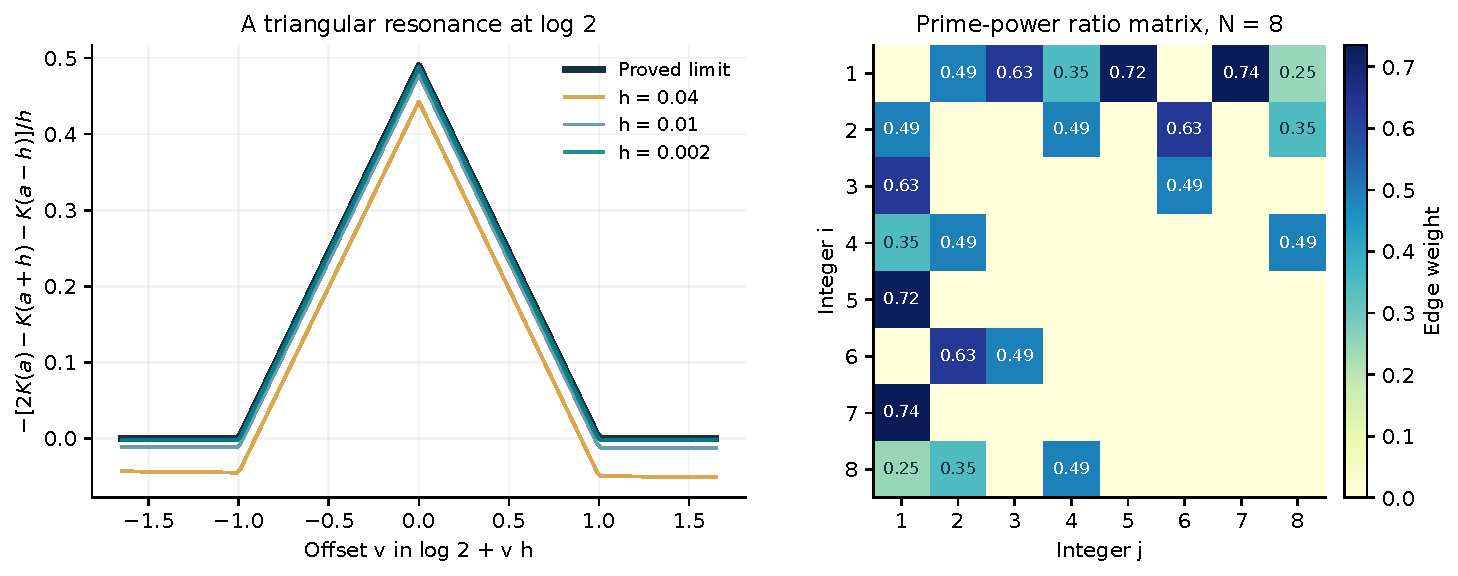
\includegraphics[width=\textwidth]{figures/resonance_and_matrix.pdf}
\caption{Left: the finite-prime expression for the zeta kernel gives a triangular
resonance near $\log2$ as the increment length shrinks. Right: the exact arithmetic
matrix on $1,\ldots,8$ has an edge precisely when the larger index is the smaller
one times a prime power. Numerical illustrations support the formulas; the proofs
do not depend on them.}
\label{fig:main}
\end{figure}

The accompanying program uses 90 decimal digits and evaluates $K_1$ by the finite
prime formula, not by truncating a zero table. It checks the covariance expansion,
the triangular profile, the matrix limit, the trace formulas for the quadratic
and cubic determinant coefficients, and diagonal sign conjugacy for the real
characters of conductors $4$ and $8$. It includes the lag $\log6$ as a negative
control. The recorded JSON contains raw numerical values and error sizes.
Numerical checks are consistency tests, not a substitute for the analytic proof.

For $N=8$ in the zeta case, the predicted quadratic coefficient is
$\tr(A^2)/2=3.1248179249011144\ldots$, and the cubic coefficient is
$\tr(A^3)/3=0.4995369779833942\ldots$. A sample of the recorded output is:
\begin{center}
\small
\begin{tabular}{@{}rrrr@{}}
\toprule
$h$ & $\max_{ij}|[\ell(I-R)-A]_{ij}|$
& $\ell^2(-\log\det R)$ &
$\ell^3[-\log\det R-S_2/\ell^2]$\\
\midrule
$10^{-3}$ & $2.9000\cdot10^{-3}$ & $3.30207484$ & $0.97361244$\\
$10^{-5}$ & $2.8655\cdot10^{-5}$ & $3.20518399$ & $0.81152305$\\
$10^{-8}$ & $2.8484\cdot10^{-8}$ & $3.16487844$ & $0.68125262$\\
$10^{-12}$ & $2.8396\cdot10^{-12}$ & $3.14831654$ & $0.61603792$\\
\bottomrule
\end{tabular}
\end{center}
The first correction is recovered at order $h$. The scaled determinant
coefficients converge much more slowly, as inverse powers of $\log(1/h)$;
the table deliberately shows that distinction.

The script \texttt{verify\_characters.py} independently evaluates the character
transfer formula for the examples of conductors $4$ and $8$, and checks their
conductor-shifted matrix limits. Its use of $L'/L(1,\chi)$ is numerical; the
symbolic transfer proof in \cref{lem:transfer} is the justification of the identity.

\section{Scope, verification status, and formalization route}

The established statements are \cref{thm:tangent,thm:triangle,thm:det,thm:gauge,thm:coalesce}
and \cref{cor:coeff}, with complete proofs above. They use RH/Dirichlet GRH as the
external theorem supplied by the pinned source, together with classical analytic
continuation, functional equations, Hadamard products, and the smoothed explicit
formula. They require neither simple zeros nor independent zero ordinates.

All asymptotics are for a fixed character and a fixed finite configuration.
Allowing $N$ or the conductor to grow would require new uniform estimates,
because neighboring prime-power thresholds become closer and local derivative
bounds change. The Gaussian processes are constructed from positive spectral
measures; no assertion of almost-periodic sample paths is made.

Two separate agent reviews checked the zeta constants, the signs of the
arithmetic correction, the uniform covariance remainder, and the determinant
argument. The real-character transfer and diagonal conjugacy were separately
checked. The new theorems have not been formalized in Lean. The archive contains
a formalization plan identifying the analytic and finite-dimensional lemmas;
it does not contain a purported completed Lean proof.

A useful formalization order is to prove the finite matrix results from the
local normal form first. The local logarithmic cusp and arithmetic ramps imply
the covariance expansion, which in turn implies the matrix and determinant laws.
The Dirichlet analytic layer supplies those local forms; the upstream theorem
supplies the real zero spectrum and hence positivity. The stochastic corollary
can be formalized last, since the arithmetic matrix and determinant results have
the deterministic Hilbert-space formulation already given.

\appendix
\section{Archive and reproducibility}

The archive contains the TeX source and compiled PDF; programs for the zeta and
character checks and for regenerating the figure; recorded JSON outputs;
the source/novelty audit; a formalization plan; and a SHA-256 manifest.
Run the commands in \texttt{README.txt} from the extracted directory.
The PDF can be built with Tectonic, or with two \texttt{pdflatex} passes,
after generating the figure.

No upstream source tree or prior packet is republished in this archive. The source
manifest records pinned URLs and hashes of the specific inspected files. This keeps
the package focused on the new proof while making its dependencies traceable.

\begin{thebibliography}{20}
\raggedright
\bibitem{grh} L. Sernau and contributors, \emph{grh-lean}, revision
\texttt{72fead102f663d5c7a407964a13dc0cf9d977207}, 25 November 2026.
\url{https://github.com/lsernau/grh-lean}.
\bibitem{statements} Same repository, \emph{grh/src/Statements.lean}, pinned revision above.
\href{https://github.com/lsernau/grh-lean/blob/72fead102f663d5c7a407964a13dc0cf9d977207/grh/src/Statements.lean}{Pinned theorem statements}.
\bibitem{main} Same repository, \emph{grh/src/Main.lean}, pinned revision above.
\href{https://github.com/lsernau/grh-lean/blob/72fead102f663d5c7a407964a13dc0cf9d977207/grh/src/Main.lean}{Pinned exported proofs}.
\bibitem{guide} Same repository, \emph{grh/GUIDE.md}, pinned revision above.
\href{https://github.com/lsernau/grh-lean/blob/72fead102f663d5c7a407964a13dc0cf9d977207/grh/GUIDE.md}{Pinned reading guide}.
\bibitem{primeerror} Same repository, \emph{grh/src/New/Reduction/Zeros/PrimeError.lean},
pinned revision above. \href{https://github.com/lsernau/grh-lean/blob/72fead102f663d5c7a407964a13dc0cf9d977207/grh/src/New/Reduction/Zeros/PrimeError.lean}{Pinned prime-remainder transform}.
\bibitem{criterion} Same repository, \emph{grh/src/New/Reduction/Zeros/Criterion.lean},
pinned revision above. \href{https://github.com/lsernau/grh-lean/blob/72fead102f663d5c7a407964a13dc0cf9d977207/grh/src/New/Reduction/Zeros/Criterion.lean}{Pinned one-sided criterion}.
\bibitem{community} Lean community, \emph{riemann-hypothesis}, theorem statements and
verification description, accessed 26 November 2026.
\url{https://github.com/leanprover-community/riemann-hypothesis}.
\bibitem{wiki} Wikipedia contributors, \emph{Riemann hypothesis}, current article
inspected 26 November 2026. Historical context only.
\url{https://en.wikipedia.org/wiki/Riemann_hypothesis}.
\bibitem{proveit} V. Reshetnikov, \emph{ProveIt: GRH research directory},
revision \texttt{2ccd1e24d0f3fa8a5268c864f66a6b1b4e2d0d59}.
\href{https://github.com/VladimirReshetnikov/ProveIt/tree/2ccd1e24d0f3fa8a5268c864f66a6b1b4e2d0d59/Analysis/GeneralizedRiemannHypothesis}{Pinned GRH research directory}.
\bibitem{cusp} Research packet \emph{dirichlet-grh-research}, section
\emph{Recovering the modulus and twist from the signed zero spectrum},
\texttt{critical-line/cusp.tex}, in \cite{proveit}.
\href{https://github.com/VladimirReshetnikov/ProveIt/blob/2ccd1e24d0f3fa8a5268c864f66a6b1b4e2d0d59/Analysis/GeneralizedRiemannHypothesis/Research/dirichlet-grh-research/critical-line/cusp.tex}{Pinned antecedent on arithmetic cusps}.
\bibitem{suzuki} M. Suzuki, \emph{Aspects of the screw function corresponding to the
Riemann zeta-function}, Journal of the London Mathematical Society \textbf{108}
(2023), 1448--1487. \url{https://doi.org/10.1112/jlms.12785}.
Preprint: \url{https://arxiv.org/abs/2206.03682}.
\bibitem{titchmarsh} E. C. Titchmarsh, revised by D. R. Heath-Brown,
\emph{The Theory of the Riemann Zeta-Function}, second edition,
Oxford University Press, 1986. Classical background for the explicit formula,
Hadamard product, and zero counting.
\bibitem{dlmf} NIST Digital Library of Mathematical Functions,
\emph{Section 25.15: Dirichlet $L$-functions}, analytic properties and
functional equations. \url{https://dlmf.nist.gov/25.15}.
\end{thebibliography}
\end{document}
